%!TEX root = r-gather.tex

\section{Experimental Results}


We have implemented this distributed algorithm along with the $r$-gather algorithm described in~\cite{Aggarwal06achievinganonymity} to compare their clustering qualities. 
%Both were coded up in Python 2.7.12 using principally, the NetworkX, NumPy, SciPy and Matplotlib packages.

%\subsection{Data Sets}

First, in order to have an intuitive understanding of its performance in the static setting, we applied our distributed algorithm to random point clouds in the plane; Figure~\ref{fig:snapshot} shows examples of resulting clusters, for $r=3,5,7,9$, on a random point cloud of size $50$.

%But in the other simulations we used all $9386$ trajectories.
%The points shown are a snapshot of the GPS co-ordinates of 1500 cars driving around Shenzhen city in China.

\begin{figure*}[htpb]
\begin{center}
\begin{tabular}{cc}
\vspace*{-8mm}
	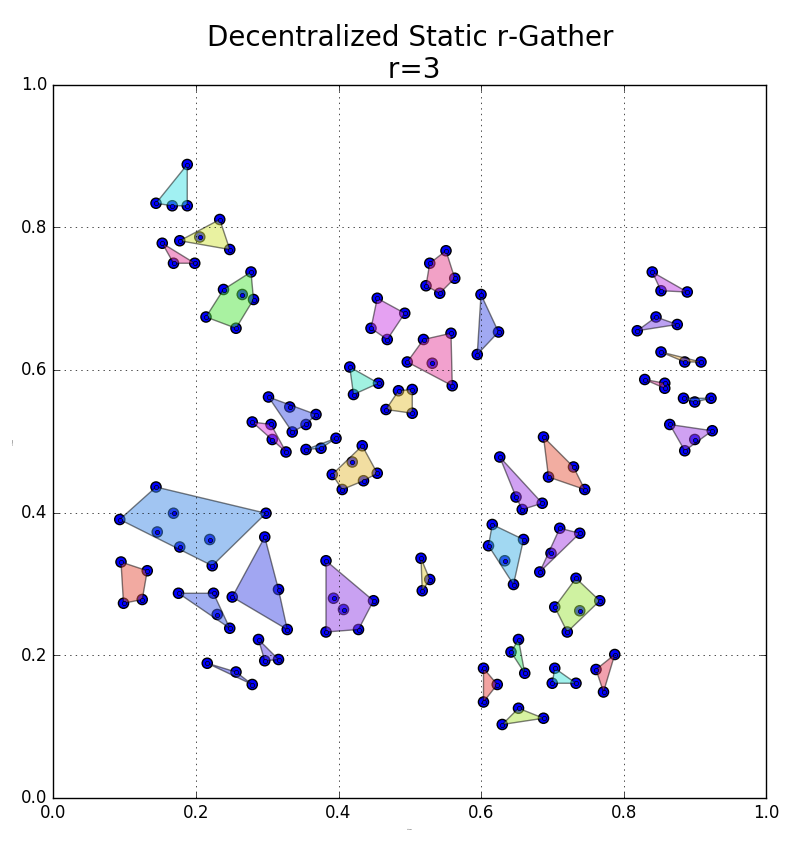
\includegraphics[scale=0.25]{figs/r3.png} &
	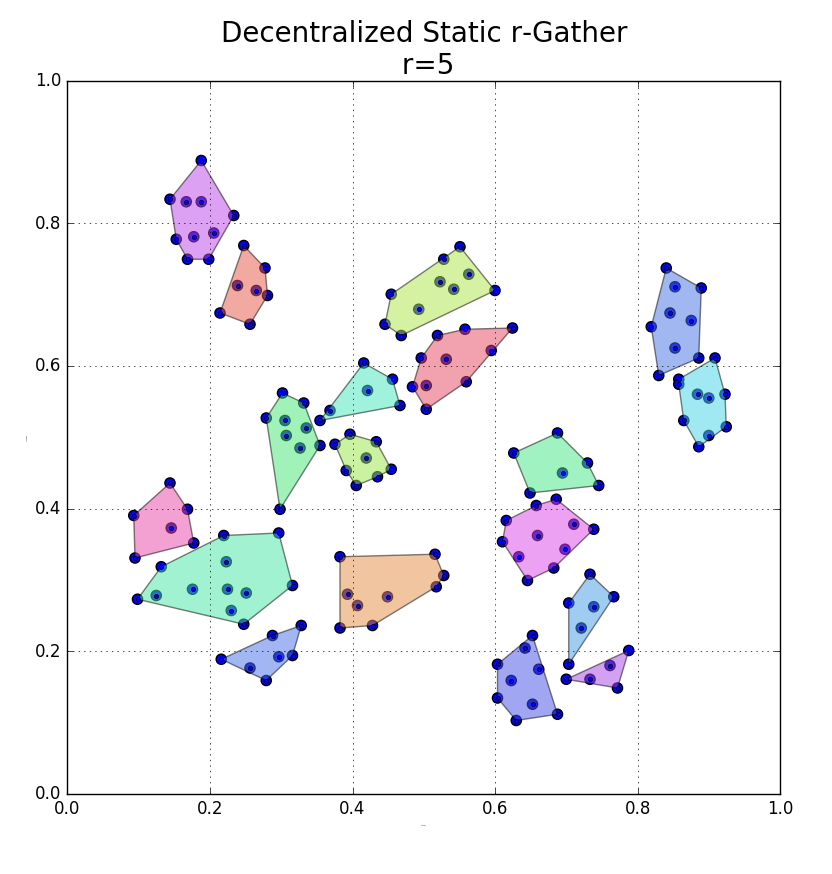
\includegraphics[scale=0.25]{figs/r5.png} \\
\vspace*{-12mm}
%\footnotesize (i) & \footnotesize (ii) \\
	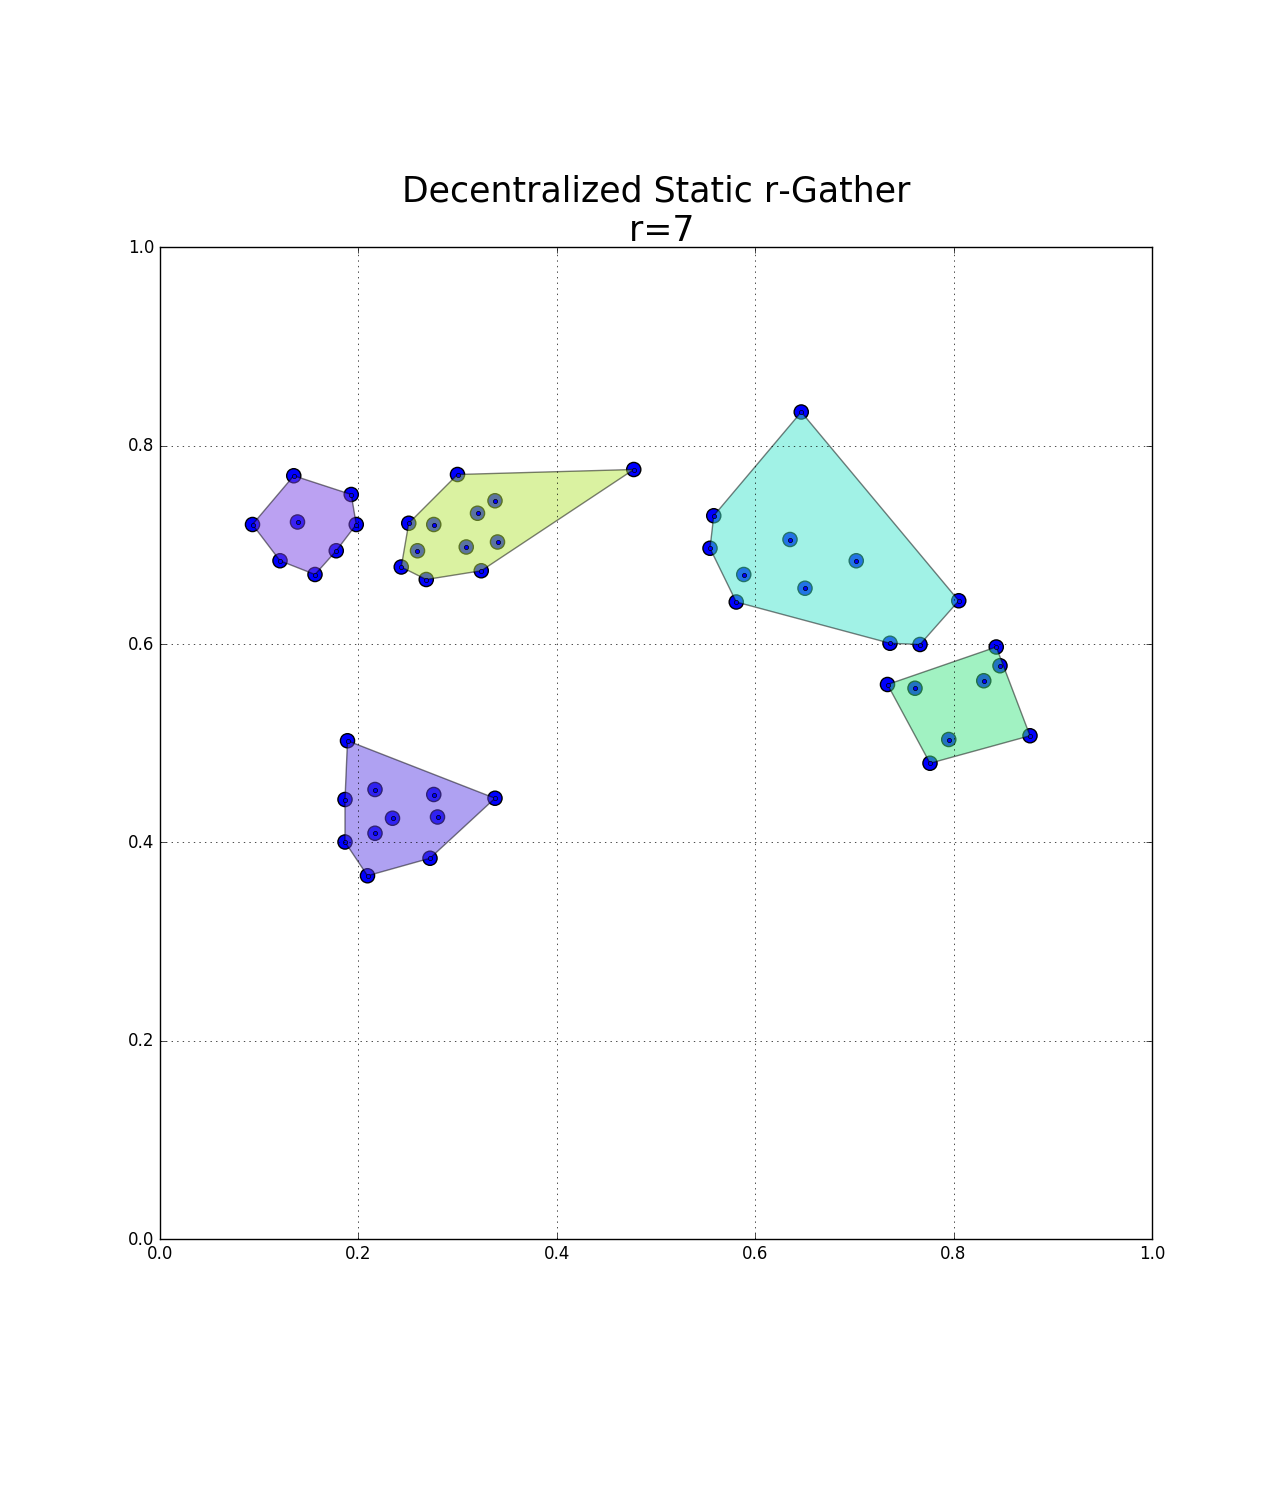
\includegraphics[scale=0.25]{figs/r7.png} & 
	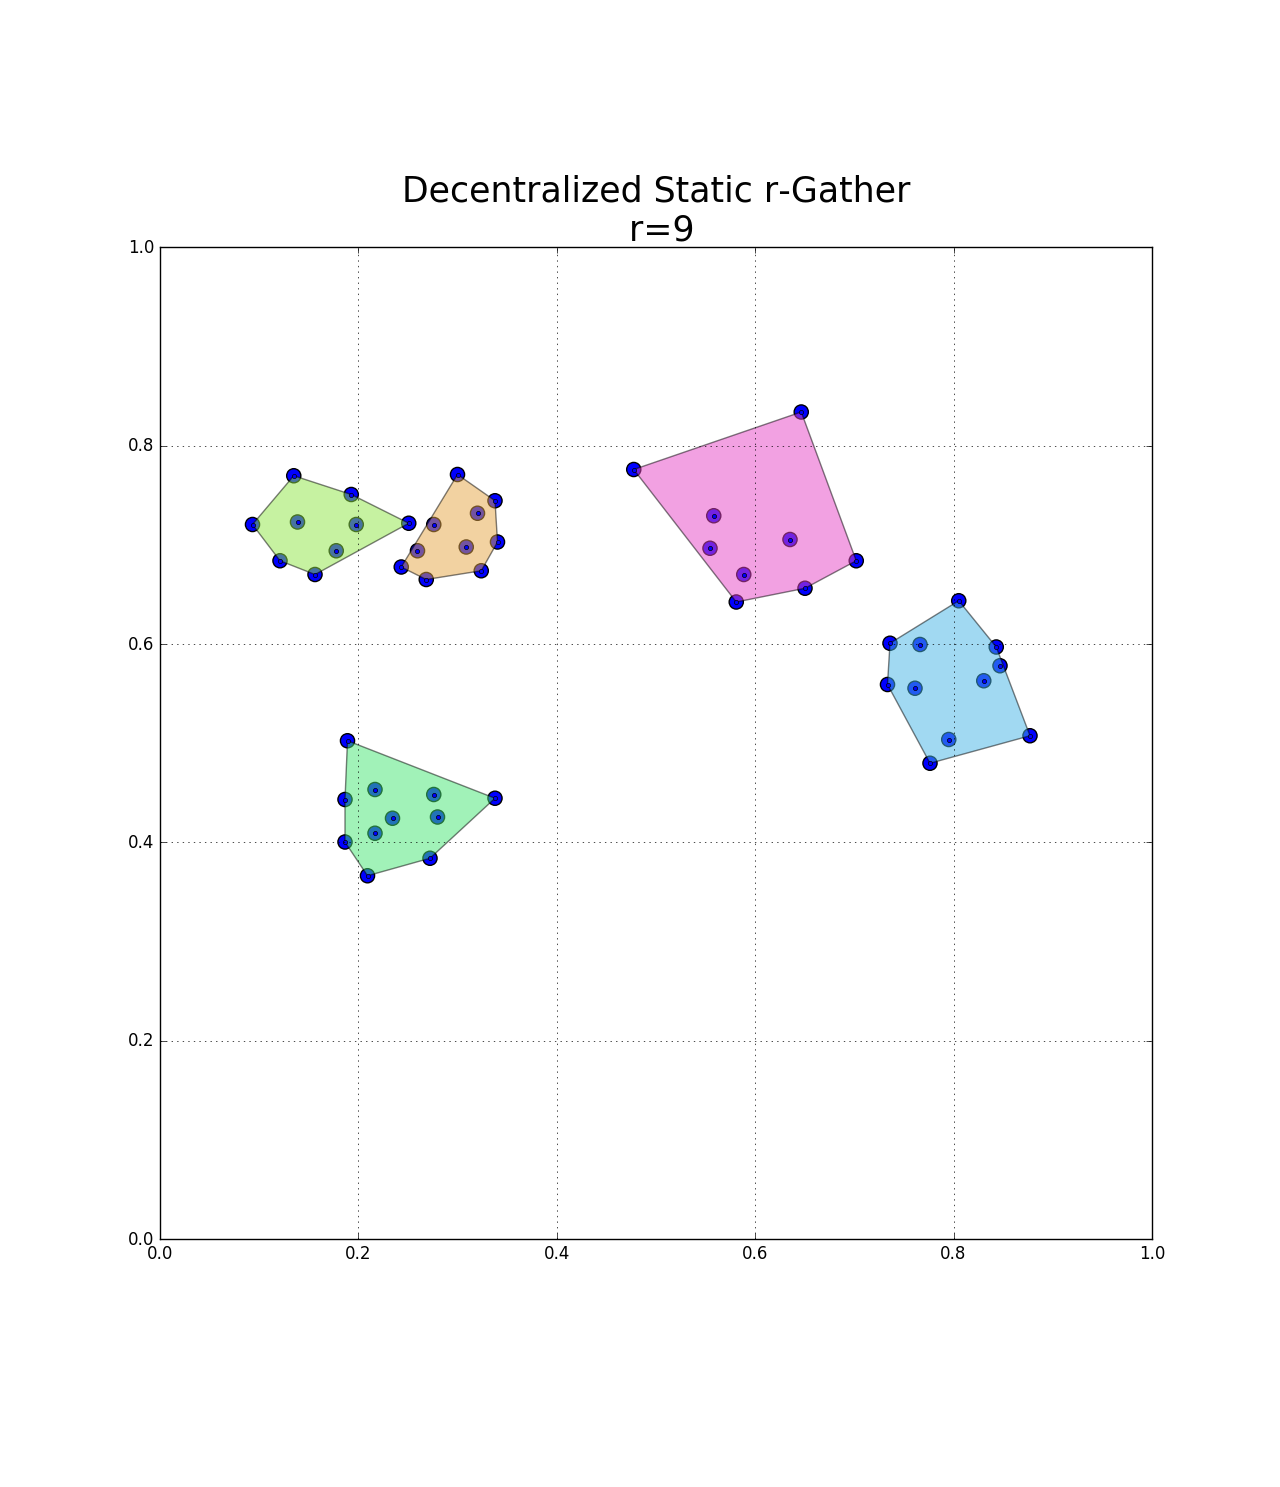
\includegraphics[scale=0.25]{figs/r9.png} 	\\
\vspace*{-6mm}
% \footnotesize (iii)& \footnotesize (iv) \\
\end{tabular}
\end{center}
%\vspace*{-6mm}
	\caption{\footnotesize The clusters produced by the distributed algorithm for a set of $50$ points uniformly randomly distributed, with $r=3$ in (top left), $r=5$ in (top right), $r=7$ in (bottom left) and $r=9$ in (bottom right) respectively. }
	\label{fig:snapshot}
%\vspace{-0.3in}
\end{figure*}

%\begin{figure}[h]
%\begin{center}
%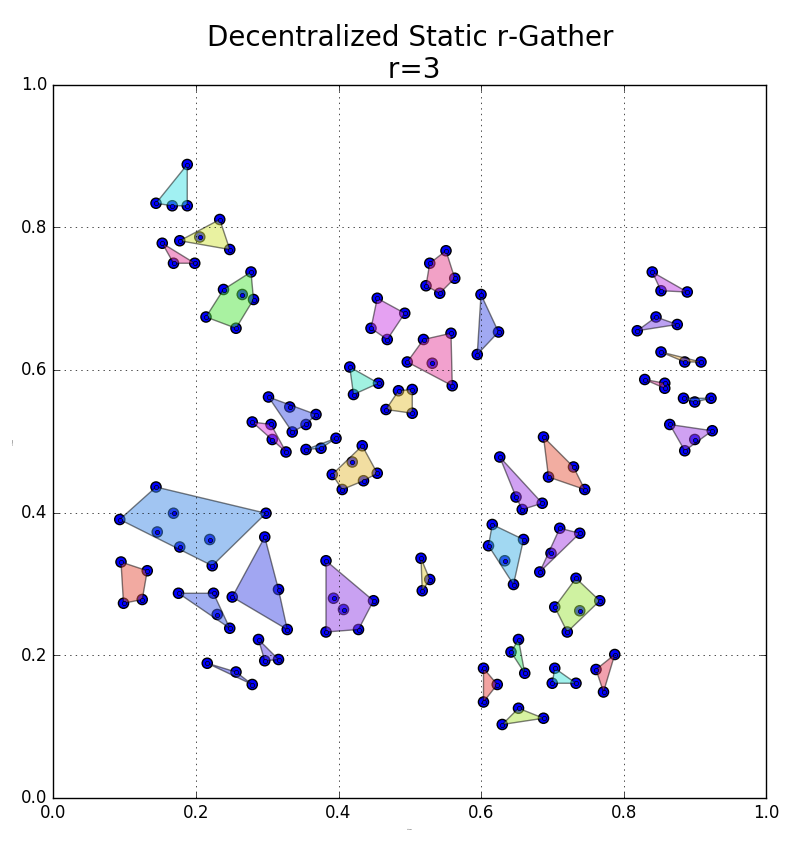
\includegraphics[width=3in]{figs/r3.png}
%\end{center}
%\end{figure}
%
%
%\begin{figure}[h]
%\begin{center}
%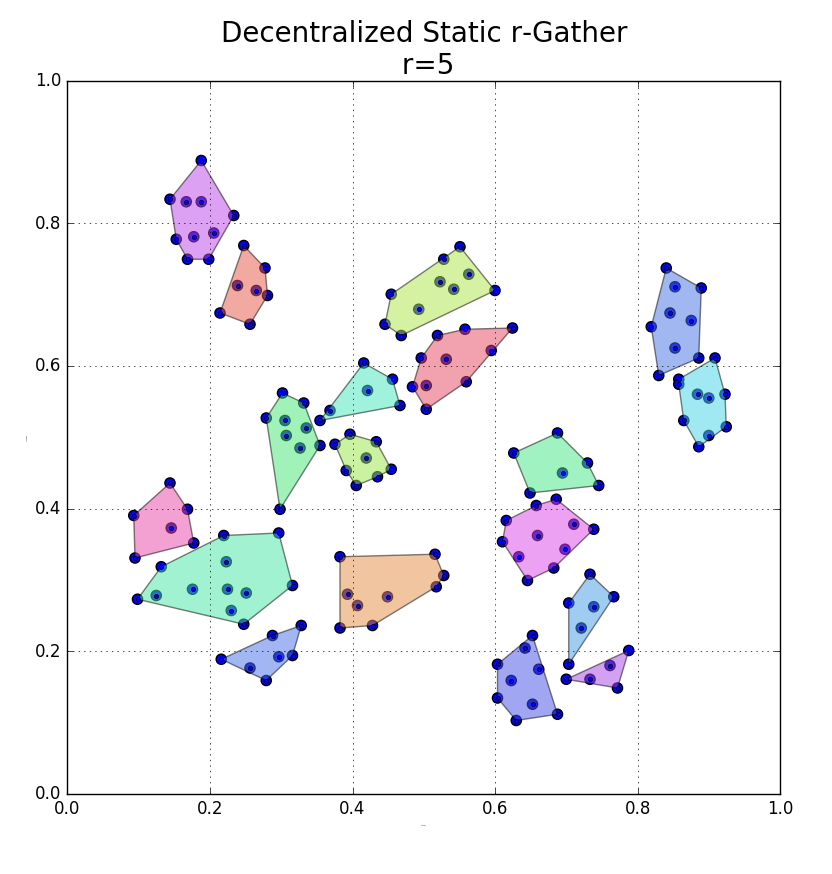
\includegraphics[width=3in]{figs/r5.png}
%\end{center}
%\end{figure}
%
%
%\begin{figure}[h]
%\begin{center}
%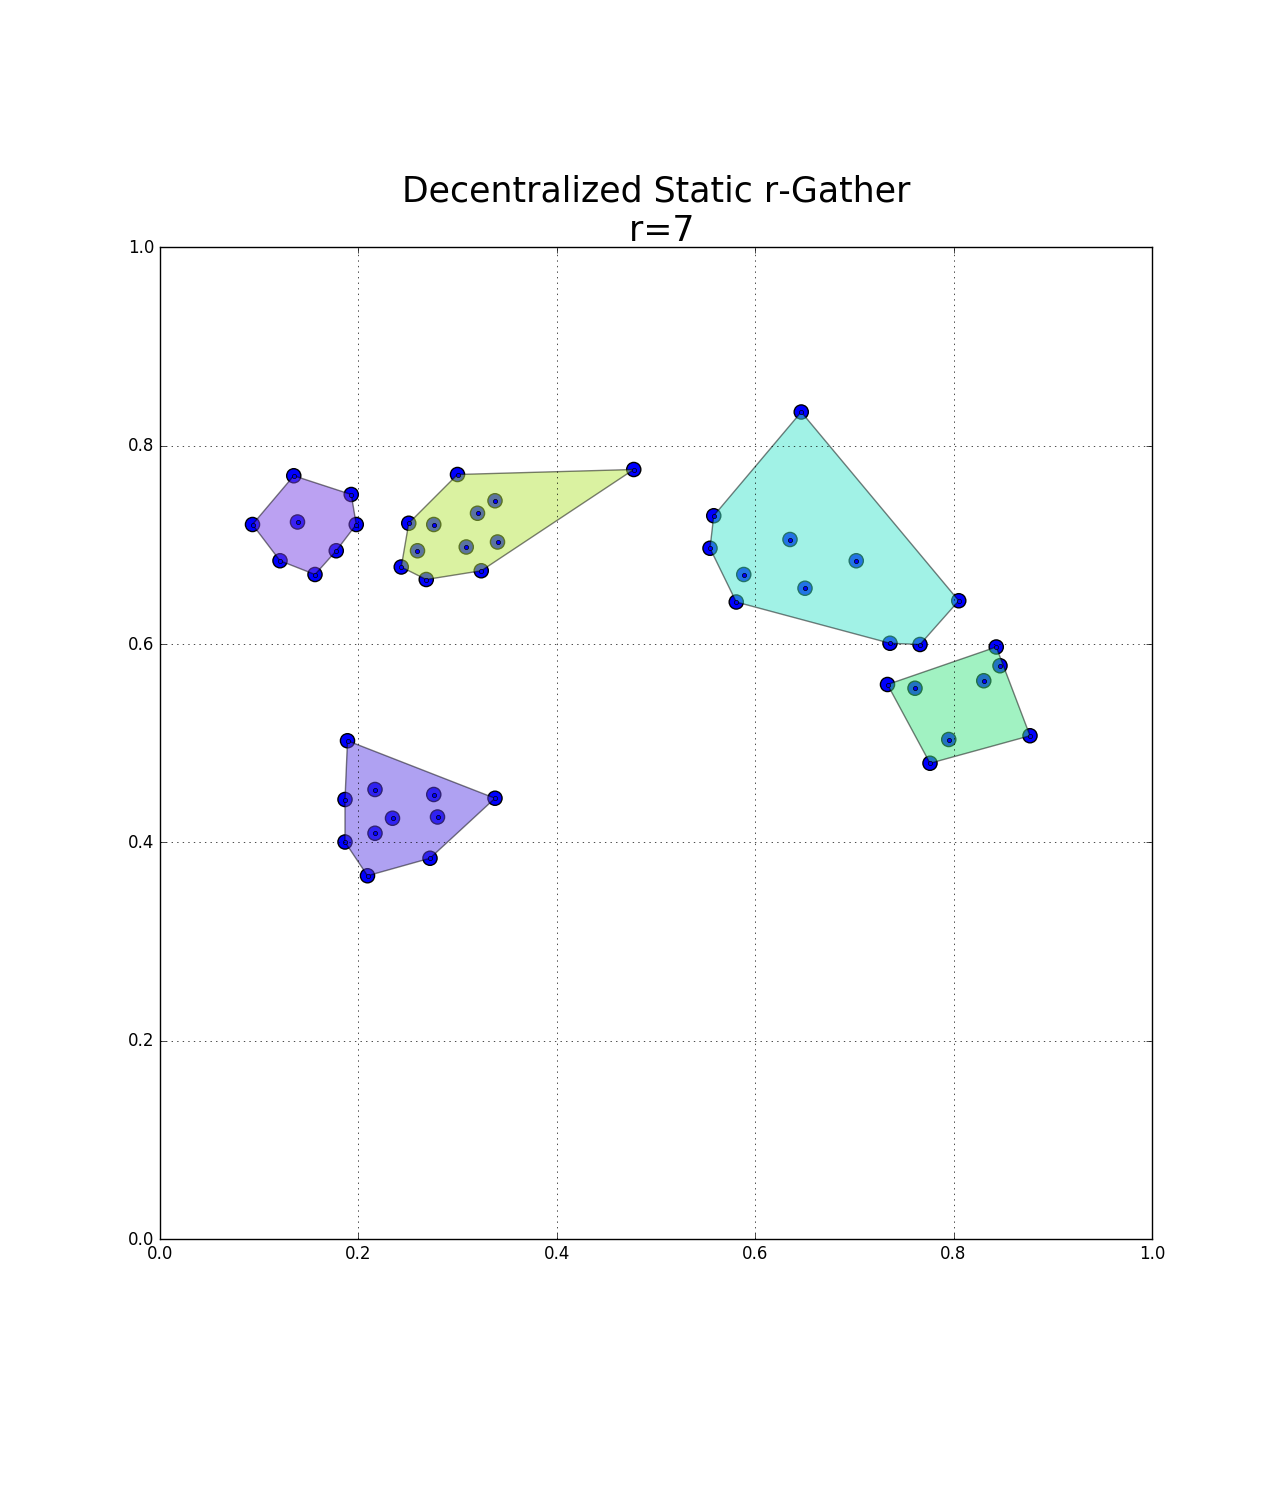
\includegraphics[width=3in]{figs/r7.png}
%\end{center}
%\end{figure}
%
%
%\begin{figure}[h]
%\begin{center}
%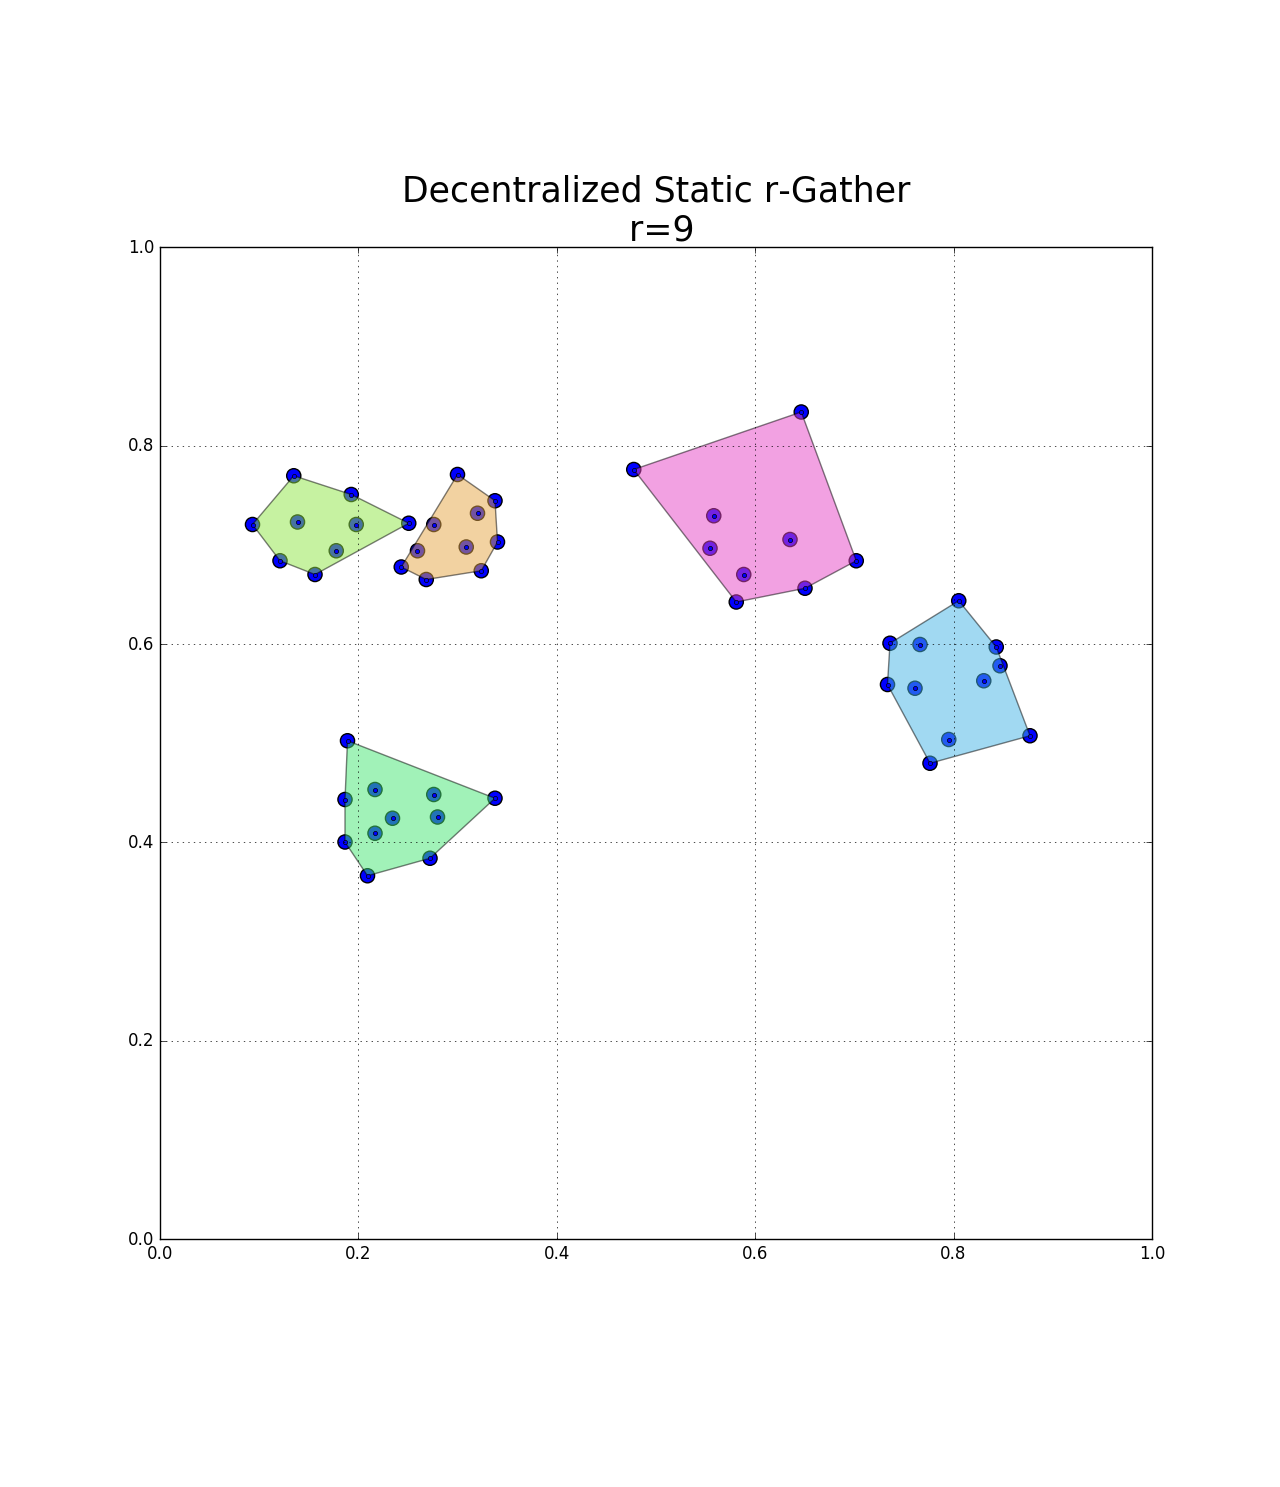
\includegraphics[width=3in]{figs/r9.png}
%\end{center}
%\end{figure}




%The $X$ and $Y$ axes in the figures above respectively denote longitude and latitude. 
%For generating these clusters and other experiments on the distributed algorithm to be described next, latitude and longitude pairs were treated simply as $x,y$ co-ordinates in $\mathbb{R}^2$. 

%\vspace{3mm}


%\subsection{Experiments}

%\vspace{3mm}


%\subsection{ Experimental Setup }        
%\vspace{2mm}


To test the quality of the clusterings generated for these algorithms for different choices of $r$, we calculated the maximum of the clusters' diameters. Our distributed algorithm has many variations depending on how exactly certain steps are performed; e.g., we can vary how one selects a good maximal independent set among the $r$-neighborhoods, $N_r(p_i)$, of the nodes $p_i\in P$. In our first implementation, we do this as follows: We compute the distance $d_r(p_i)$ from $p_i$ to its $r$th nearest neighbor, for each $p_i$; we then add to the independent set that $r$-neighborhood $N_r(p_i)$ that minimizes $d_r(p_i)$, remove the points $p_i$ and $N_r(p_i)$ from $P$, and then repeat this selection process, until no $r$-neighborhoods remain.  In another variant of our implementation, we select the maximal independent set of $r$-neighborhoods greedily (with preference to those of smallest diameter); in fact, we repeat the process $K$ times (by default, we chose $K=20$), and select the best solution from the multiple runs.
%% Joe:  Question for Gaurish:  why repeat?  Is there an element of random choice in the greedy algorithm? If so, we need to clarify this!  Also, what does ``best'' mean? (the one whose largest diameter is smallest, I assume?)

% Use to blank out text portions that are old, but not discarded                                                                                  \newcommand{\old}[1]{{}}
\old{
Given a graph G=(V,E), find a maximal set in G.
0. initialize I = empty.
1. pick a node, v, in V at random; place it in I
2. remove v and its neighbors from V.
3. if V is nonempty, go to 1

It this right?
(I just looked at the source code:
https://networkx.github.io/documentation/networkx-1.9.1/_modules/networkx/algorithms/mis.html#maximal_independent_set   )

We should make this more clear in the text, of course.

There are many other ways one can imagine to find a maximal indep set.

A very natural greedy is this:  Pick a lowest degree node v in V to add to I (then remove it, and its neighbors, repeat).
We need a rule to break ties for lowest degree:  in our setting, we could do so in favor of smallest d_r(v).

Note too, that instead of using d_r(v) as a measure of "size" (radius, or diameter), we could use the actual diameter of
the r-neighborhood, N_r(v).

I would suggest that we try out these other variants.....
}

For each clustering algorithm, we calculate the following two statistics:
\bitem
\item  The maximum, over all clusters, of the diameters of the clusters.
\item  The $90$th percentile of the diameters of the clusters.
%\item  The  maximum over all clusters, the $90$th percentile of point-distances within a cluster.
\eitem
We also plot the value of $d_r^{\max}=\max_i d_r(p_i)$, which we know (Observation~\ref{obs:lower-bound}) is a lower bound on the optimal diameter, $D_{OPT}$, in an $r$-gather solution.

We ran our algorithms on a data set of the GPS coordinates of $9386$
taxicabs in Shenzhen (China), sampled at 5 minute intervals over one
full day.
Figure~\ref{fig:comparison} shows the results of our algorithm, in comparison
to~\cite{Aggarwal06achievinganonymity} and $d_{r}^{\max}$ as a baseline, on a snapshot containing $60$ random users from the dataset. Figure~\ref{fig:comparison-90} shows the $90\%$ percentile results.  

\begin{figure}[h]
\begin{center}
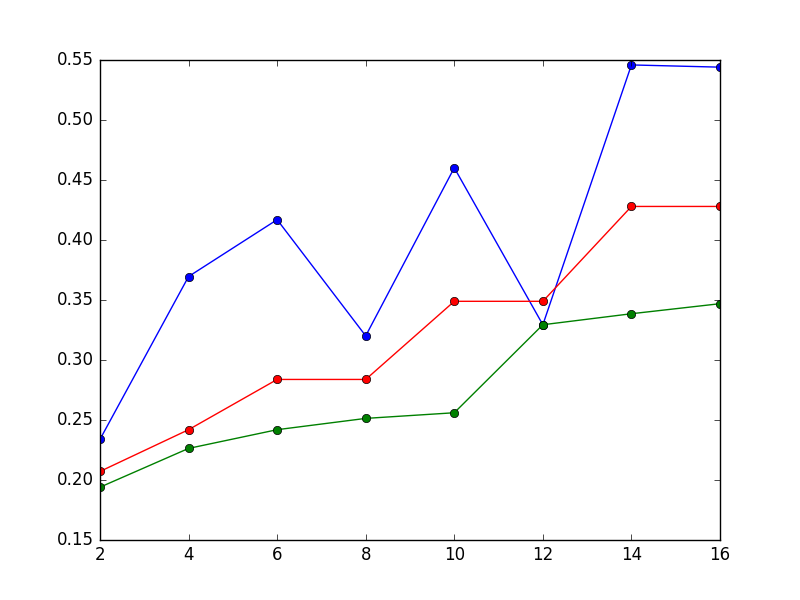
\includegraphics[width=3in]{figs/figure_1.png}
\caption{Maximum cluster diameter. Blue: approximation algorithm from~\cite{Aggarwal06achievinganonymity}; Red: distributed algorithm; Green: $d_{r}^{\max}$.}\label{fig:comparison}
\end{center}
\end{figure}


\begin{figure}[h]
\begin{center}
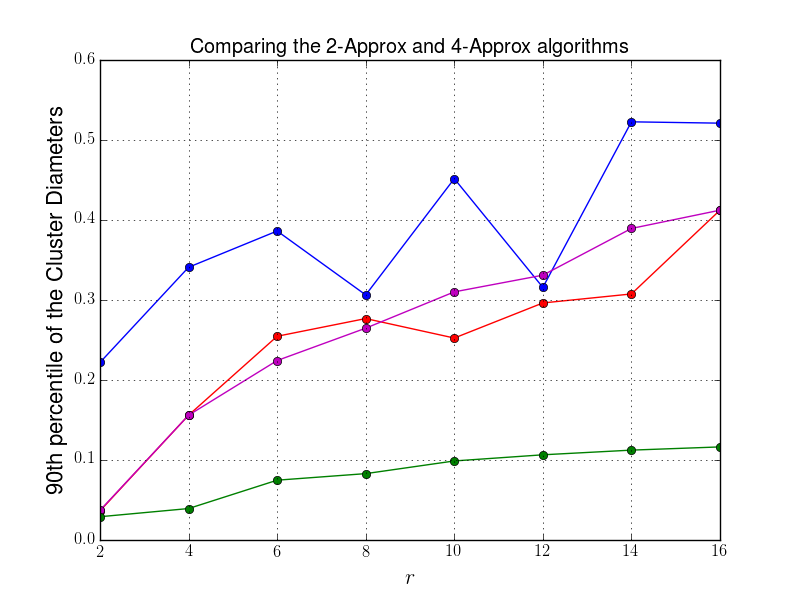
\includegraphics[width=3in]{figs/90thpercentile_60Cars.png}
\caption{$90\%$ percentile of all cluster diameter. Blue: approximation algorithm from~\cite{Aggarwal06achievinganonymity}; Red: distributed algorithm; Green: $d_{r}^{\max}$; Magenta: the distributed algorithm with the best maximal independent set run over $20$ iterations.}\label{fig:comparison-90}
\end{center}
\end{figure}

Figure~\ref{fig:large} shows results on a larger dataset of $1500$
mobile users; the distributed algorithm still performs well. Figure~\ref{fig:large-90} shows the $90\%$ percentile results.  


\begin{figure}[h]
\begin{center}
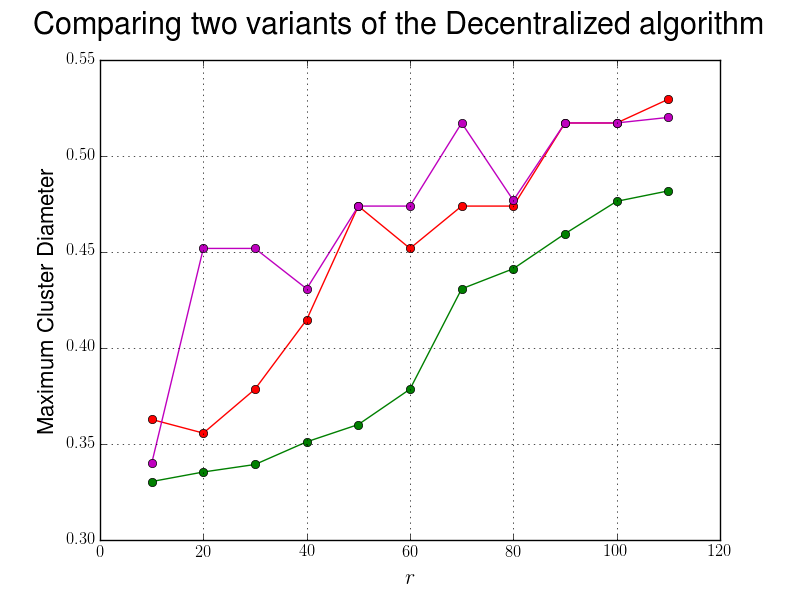
\includegraphics[width=3in]{figs/cars1500_4Approx.png}
\caption{Maximum cluster diameter on a snapshot of 1500 mobile users. Red: distributed algorithm; Green: $d_{r}^{\max}$; Magenta: the distributed algorithm with the best maximal independent set run over $20$ iterations.}\label{fig:large}
\end{center}
\end{figure}

\begin{figure}[h]
\begin{center}
\includegraphics[width=3in]{figs/90thpercentile_1500cars.png}
\caption{$90\%$ percentile of all cluster diameter. 
Red: distributed algorithm; Green: $d_{r}^{\max}$; Magenta: the distributed algorithm with the best maximal independent set run over $20$ iterations.}\label{fig:large-90}
\end{center}
\end{figure}

%\vspace{3mm}

%\bitem
%\item  The maximum over all clusters, the diameter of a cluster.  
%\item  The maximum over all clusters, the $90$th percentile of point-distances within a cluster.
%\eitem
%\vspace{3mm}

%\vspace{3mm}




%\vspace{20mm}




%We implemented the distributed algorithm and compared it with~ \cite{Aggarwal06achievinganonymity} and with the lower bound of $d_{r}^{\max}$  on real location data from a trajectory dataset of 9000 mobile users in Shenzen city in china. 

%
%\begin{figure}[h]
%\begin{center}
%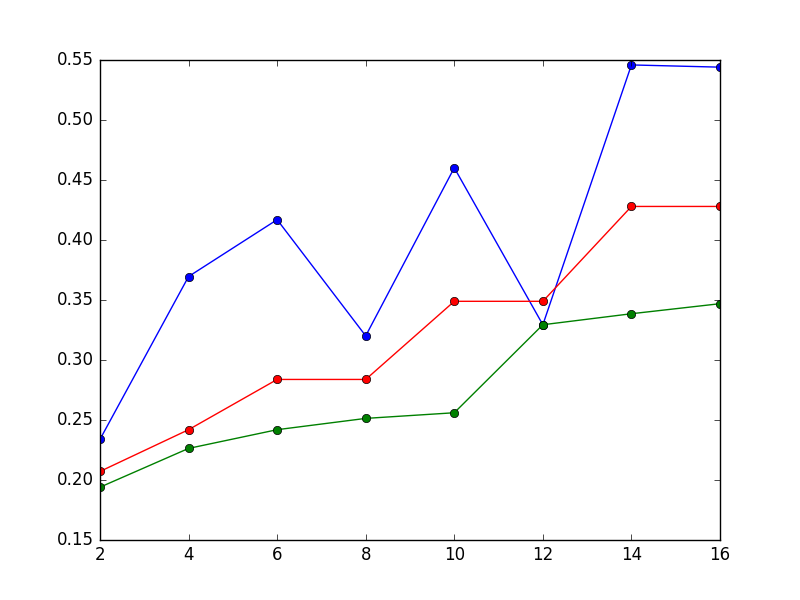
\includegraphics[width=3in]{figs/figure_1.png}
%\caption{Max cluster diameter. Black curve: approximation algorithm from~\cite{Aggarwal06achievinganonymity};
%  Red curve: distributed algorithm; Green curve: $d_{r}^{\max}$.}\label{fig:comparison}
%\end{center}
%\end{figure}






%We implemented the distributed algorithm and compared it with~\cite{Aggarwal06achievinganonymity} and with the lower bound of $d_{r}^{\max}$ on real location data from a trajectory dataset of 9000 mobile users in Shenzen city in china. 
Our main observations are:

\begin{itemize}
\item Our distributed algorithm usually produces better results than the $2$-approximation algorithm of~\cite{Aggarwal06achievinganonymity} in practice, although the approximation bound for the distributed algorithm is worse in theory.
\item The distributed algorithm runs faster and therefore can be run on larger datasets
\item The results (maximum cluster diameters) are close to the lower bound of $d_{r}^{\max}$.
\end{itemize}


%
%\begin{figure}[h]
%\begin{center}
%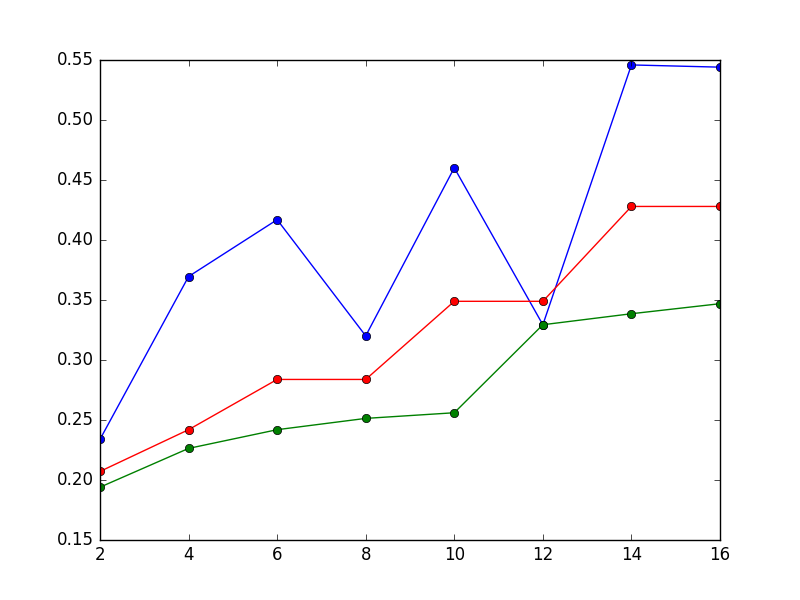
\includegraphics[width=3in]{figs/figure_1.png}
%\caption{Max cluster diameter. Black curve: approximation algorithm from~\cite{Aggarwal06achievinganonymity};
%  Red curve: distributed algorithm; Green curve: $d_{r}^{\max}$.}\label{fig:comparison}
%\end{center}
%\end{figure}

